 \chapter{Introduction}
 
\pagenumbering{arabic}
\setcounter{page}{1}

Molecular imaging has provided science with great advances during it's history, such as X-ray crystallography determining the helical structure of DNA in 1953~\cite{watson_molecular_1953} and structure of myoglobin and haemoglobin in 1962~\cite{kendrew_x-ray_1957}.
The \gls{caeis} at the University of Melbourne is an ongoing project that aims to develop a source capable of achieving the `holy grail' of scientific imaging, the `molecular movie'~\cite{dwyer_femtosecond_2006,sciaini_femtosecond_2011}.
A \gls{caeis} also has potential applications with \gls{fib} techniques~\cite{mcclelland_bright_2016}, and as particle source for accelerators such as synchrotrons and \glspl{xfel} for \gls{cdi} of non-crystalline targets~\cite{van_oudheusden_electron_2007, zhu_future_2015, mcculloch_cold_2016}.



{\color{red}
Some kind of introduction for everything will go here.

Motivate CAES. Imaging of things is important. Membrane proteins, cystallisation. What else can we image with it? What else can we study with it? Ion source.

Briefly motivate part 1 and part 2.}

\section{Making the `Molecular Movie'}

Being able to observe molecular dynamics at an atomic spatial and temporal scale could provide great insight into some of the basic processes of biology and chemistry.
The fabled `molecular movie' refers to capturing the atomic motions of molecular systems as they undergo some transition such as a chemical reaction, protein folding or melting.
Molecular movies could provide greater understanding of important biological reactions such as photosynthesis or oxygen transport by haemoglobin.

One of the stepping stones towards molecular movies is single-shot imaging of non-crystalline molecules which would allow structural determination of membrane proteins, an essential step in rational drug design~\cite{hardy_atomic_1987, barrett_discovering_1999, pinto_influenza_1992}.
One of the main techniques in stuctural determination of crystalline targets is electron diffraction which, along with X-ray and neutron methods~\cite{cullity_elements_2001,bacon_x-ray_2013}, has be utilised in structural determination of many materials with atomic resolution.
Continuing research into real-space and diffraction imaging techniques is aiding in the understanding of a growing range of samples as well as providing new types of information on the sample under investigation.

Ultrafast imaging techniques are a relatively recent development and they provide the opportunity to study electronic and atomic dynamics.
Ultrafast techniques also provide an avenue for the imaging of structures that, to date, cannot be imaged by cyrstallographic techniques as some of these techniques should be applicable to uncrystallised samples with imaging being faster than damage processes~\cite{gaffney_imaging_2007,barty_ultrafast_2008,miao_beyond_2015}.
In the past the greatest success with structural determination has been acheived with crystallography which is limited by to samples that can be crystallised.
There are a large number of biological proteins of interest, particularly membrane proteins, that cannot be crystallised and developements in ultrafast imaging techniques is providing a route towards structural determination without crystallisation~\cite{dauter_current_2006,levitt_nature_2009}, cryogenic electron microscopy is also making headway in this area~\cite{henderson_model_1990,zhou_towards_2008}.
Both X-ray and electron imaging techniques are limited by the capabilities of their sources which are undergoing continual developement, in the realms of fundamental physics and engineering.
The techniques using X-rays and electrons each have different advantages and disadvantages with regards to dynamic imaging and structural determination and they often give complementary information.

One proposed method for generating molecular movies involves using a high-brightness ultrashort-duration beam source, such as a \gls{xfel} or future-\gls{caes}, to perform \gls{cdi} on individual molecules~\cite{chapman_femtosecond_2006,dwyer_femtosecond_2006,gaffney_imaging_2007}.
The individual molecules would be dropped one-by-one infront of the illuminating bunches which would be short enough that imaging is completed before damage from the illumination affects the diffraction pattern, see Figure~\ref{figure:molecule_cdi}.
Dynamic processes, such as phase transitions, melting, and pumped vibrational modes, can be studied with this technique if the process can be triggered, say with a precisely timed laser pulse, and by varying the delay between triggering the process and imaging the molecule a `movie' can be constructed.
The random orientation of molecules as they are imaged can be dealt with algorithmically~\cite{yefanov_orientation_2013}.

\begin{figure}
    \center
    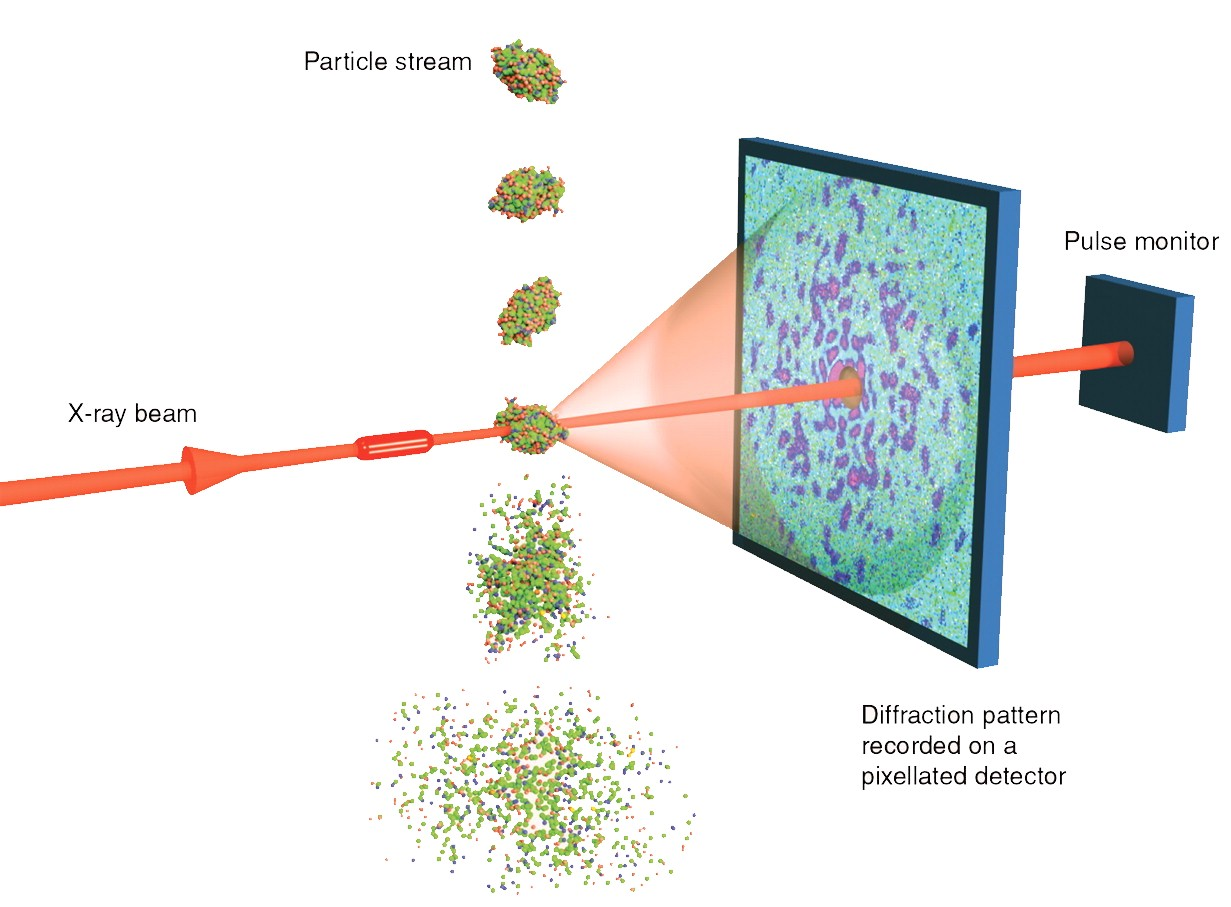
\includegraphics[width=0.65\linewidth]{0intro/Figs/single_molecule_cdi.jpg}
    \caption{Structural determination of single molecules should be possible if a sufficiently bright and short pulse of X-rays is used image the molecule before damage affects the diffraction patter prduced. Electrons could be used in place of X-rays if a suitable source can be developed. Image adapted from Reference~\cite{gaffney_imaging_2007}}
    \label{figure:molecule_cdi}
\end{figure}

Some recent results from X-ray sources are well on the way to producing molecular movies~\cite{pande_femtosecond_2016,nango_three-dimensional_2016}.

\subsection{Imaging Targets}

Membrane proteins.
Chemical reactions.


\subsection{Requirements}

Ultra-fast, single-shot, orientation, flux, coherence.

\subsection{X-rays vs. Electrons}

Interaction strength
Wavelength

Current source options

Synchrotrons
XFELs

Photocathode sources
CAESs

\section{Cold-atom electron and ion sources}

The research described by this thesis is part of an ongoing effort to develope an alternative source of electrons and ions that extracts the charged particles from a laser cooled atomic cloud.
Initially the aim of the project was to create ultrafast coherent electron bunches for use in diffraction imaging in a similar way to ultrafast X-ray pulses however it was later realised that \gls{caes} could also serve as an injection source for particle accelerators.
It has also become apparent that by simply reversing the polarity of the accelerator the source can generate high quality ion bunches with similar properties to the electron bunches thus providing a new source for use in ion microscopy and nano-fabrication.

Cold-atom sources operate by carefully ionising atoms in a \gls{mot} such that the resulting ions and electrons are cold and thus the bunches accelerated from those clouds have low emittance and high coherence.
The low transverse temperature of ions and electrons produced by a \gls{caeis} is one of the main advantages of this source however the source also allows for the production ultrafast bunches, arbitrarily shaped bunches and these techniques are applicable to any of the many atomic species that can be laser cooled and trapped.

A \gls{caes} can be thought of as a photocathode electron source with the solid cathode replaced with an ultracold gas which provides the \gls{caes} with a few advantages such as the high quantum efficiency achievable, and near-threshold ionisation producing colder electrons than those from other photocathode sources~\cite{engelen_effective_2014}.
The simplicity of the interactions between photons and atoms allows for the high quantum efficiency to be achieved.
In comparison, in solid cathodes the atoms surrounding a photonic interaction complicate the ionisation and electron extraction processes.
An isolated atom, such as that in the ultracold gas, that interacts with a photon has a much more limited range of potential outcomes, absorption of the photon, radiative decay or ionisation, each with well understood probabilities thus allowing the optimisation of the quantum efficiency~\cite{baranov_field_1994}.

Another advantage of gas photocathodes over solid ones is the lack of optically induced damage from high-intensity laser-fields.
Solid cathodes undergo constant degradation due to the strong fields used and require regular replacement~\cite{dowell_results_1995} whereas the gaseous target in a \gls{caes} is renewed with every bunch produced.

One of the major advantages of \glspl{caeis} is the low temperature of the source which is due to the careful ionisation of the atoms trapped within the \gls{mot}.
The ultracold atoms trapped in the \gls{mot} have temperatures around \unit[100]{$\muup$K} but after ionisation the electrons have temperatures determined by the excess energy from the ionisation process~\cite{engelen_high-coherence_2013,engelen_analytical_2014,sparkes_high-coherence_2014,speirs_identification_2017}.
Precise control over the ionisation is possible due to the well understood physics and high quality lasers available, so it is possible to minimise the excess energy from the ionisation process and electrons produced can have transverse temperature as low as \unit[$\sim$10]{K}~\cite{saliba_spatial_2012}.
Unlike electrons ions produced by the source have their initial temperature determined predominantly by the temperature of the trapped atoms before ionisation, \unit[100]{$\muup$K}, with an ion temperature around \unit[1]{mK}~\cite{debernardi_measurement_2011,murphy_detailed_2014}.

\subsection{Developments}

Arbitrary shaping, charged partical dynamics, diffraction.
\subsection{Ion Source}

\section{Thesis Outline}

\subsection{Part I}

\subsection{Part II}
